% Credits are indicated where needed. The general idea is based on a template by Vel (vel@LaTeXTemplates.com) and Frits Wenneker.

\documentclass[11pt, a4paper]{article} % General settings in the beginning (defines the document class of your paper)
% 11pt = is the font size
% A4 is the paper size
% “article” is your document class

%----------------------------------------------------------------------------------------
%	Packages
%----------------------------------------------------------------------------------------

% Necessary

\usepackage{listings}
\usepackage[german,english]{babel} % English and German language 
\usepackage{booktabs} % Horizontal rules in tables 
% For generating tables, use “LaTeX” online generator (https://www.tablesgenerator.com)
\usepackage{comment} % Necessary to comment several paragraphs at once
\usepackage[utf8]{inputenc} % Required for international characters
\usepackage[T1]{fontenc} % Required for output font encoding for international characters

% Might be helpful
\usepackage{amsmath,amsfonts,amsthm} % Math packages which might be useful for equations
\usepackage{tikz} % For tikz figures (to draw arrow diagrams, see a guide how to use them)
\usepackage{tikz-cd}
\usetikzlibrary{positioning,arrows} % Adding libraries for arrows
\usetikzlibrary{decorations.pathreplacing} % Adding libraries for decorations and paths
\usepackage{tikzsymbols} % For amazing symbols ;) https://mirror.hmc.edu/ctan/graphics/pgf/contrib/tikzsymbols/tikzsymbols.pdf 
\usepackage{blindtext} % To add some blind text in your paper
\usepackage{placeins}

%---------------------------------------------------------------------------------
% Additional settings
%---------------------------------------------------------------------------------

%---------------------------------------------------------------------------------
% Define your margins
\usepackage{geometry} % Necessary package for defining margins

\geometry{
	top=2cm, % Defines top margin
	bottom=2cm, % Defines bottom margin
	left=2.2cm, % Defines left margin
	right=2.2cm, % Defines right margin
	includehead, % Includes space for a header
	%includefoot, % Includes space for a footer
	%showframe, % Uncomment if you want to show how it looks on the page 
}

\setlength{\parindent}{15pt} % Adjust to set you indent globally 

%---------------------------------------------------------------------------------
% Define your spacing
\usepackage{setspace} % Required for spacing
% Two options:
\linespread{1.5}
%\onehalfspacing % one-half-spacing linespread

%----------------------------------------------------------------------------------------
% Define your fonts
\usepackage[T1]{fontenc} % Output font encoding for international characters
\usepackage[utf8]{inputenc} % Required for inputting international characters

\usepackage{XCharter} % Use the XCharter font


%---------------------------------------------------------------------------------
% Define your headers and footers

\usepackage{fancyhdr} % Package is needed to define header and footer
\pagestyle{fancy} % Allows you to customize the headers and footers

%\renewcommand{\sectionmark}[1]{\markboth{#1}{}} % Removes the section number from the header when \leftmark is used

% Headers
\lhead{} % Define left header
\chead{\textit{}} % Define center header - e.g. add your paper title
\rhead{} % Define right header

% Footers
\lfoot{} % Define left footer
\cfoot{\footnotesize \thepage} % Define center footer
\rfoot{ } % Define right footer

%---------------------------------------------------------------------------------
%	Add information on bibliography

\usepackage{natbib} % Use natbib for citing
\usepackage{har2nat} % Allows to use harvard package with natbib https://mirror.reismil.ch/CTAN/macros/latex/contrib/har2nat/har2nat.pdf

% For citing with natbib, you may want to use this reference sheet: 
% http://merkel.texture.rocks/Latex/natbib.php

%---------------------------------------------------------------------------------
% Add field for signature (Reference: https://tex.stackexchange.com/questions/35942/how-to-create-a-signature-date-page)
\newcommand{\signature}[2][5cm]{%
  \begin{tabular}{@{}p{#1}@{}}
    #2 \\[2\normalbaselineskip] \hrule \\[0pt]
    {\small \textit{Signature}} \\[2\normalbaselineskip] \hrule \\[0pt]
    {\small \textit{Place, Date}}
  \end{tabular}
}

\usepackage{listings}
\usepackage{xcolor}

\definecolor{codegreen}{rgb}{0,0.6,0}
\definecolor{codegray}{rgb}{0.5,0.5,0.5}
\definecolor{codepurple}{rgb}{0.58,0,0.82}
\definecolor{backcolour}{rgb}{0.95,0.95,0.92}

\lstdefinestyle{mystyle}{
	backgroundcolor=\color{backcolour},   
	commentstyle=\color{codegreen},
	keywordstyle=\color{magenta},
	stringstyle=\color{codepurple},
	basicstyle=\ttfamily\scriptsize,
	breakatwhitespace=false,         
	breaklines=true,                 
	captionpos=t,                    
	keepspaces=true,                 
	numbers=none,                    
	numbersep=5pt,                  
	showspaces=false,                
	showstringspaces=false,
	showtabs=false,                  
	tabsize=2
}

\lstset{style=mystyle}
%---------------------------------------------------------------------------------
%	General information
%---------------------------------------------------------------------------------
\title{Automated Rule learning for PRAM} % Adds your title
\author{
Ashish Jha % Add your first and last name
    %\thanks{} % Adds a footnote to your title
    %\institution{YOUR INSTITUTION} % Adds your institution
  }

\date{} % Adds the current date to your “cover” page; leave empty if you do not want to add a date


%---------------------------------------------------------------------------------
%	Define what’s in your document
%---------------------------------------------------------------------------------

\begin{document}


% If you want a cover page, uncomment "\input{coverpage.tex}" and uncomment "\begin{comment}" and "\end{comment}" to comment the following lines
%\input{coverpage.tex}

%\begin{comment}
\maketitle % Print your title, author name and date; comment if you want a cover page 



%----------------------------------------------------------------------------------------
% Introduction
%----------------------------------------------------------------------------------------
\setcounter{page}{1} % Sets counter of page to 1

\section{Introduction} % Add a section title
%\subsection{Highlighting} % Add a subsection
One of the core component of \textbf{PRAM} \cite{pram} Simulation Engine is \textbf{Rules} which forms the basis for redistribution of mass among groups. PRAM models have rules that are mutually exclusive condition and each condition is associated with a probability distribution. Currently, these rules have to be manually created based on modeler's judgment. Given the amount of historical data we have about events, we can also learn these rules by analyzing the statistical dependency between these sequential events. These events are partially stochastic in nature. We have developed a data-driven approach for extracting rules directly from observed data by exploiting these dependencies between them

%\LaTeX allows you to highlight text in various ways: \textbf{bold}, \textit{italics}, with \textsc{small caps} or \texttt{as a coding font}.\footnote{ This command adds a footnote to your text.} 

%\subsection{Citing} % Add another subsection
%Citing in \LaTeX is easy. You could easier cite with the text flow like this ``Referring to \citet{collier2004greed} ...''  or at the end of the sentence \cite{collier2004greed}. You can also cite pages like this \citep[55]{collier2004greed}. If you want to add an additional note, you might want to do it this way \citep[cp.][22]{collier2004greed} or like this \citep[cp.][]{collier2004greed}.\\
%\blindtext % Adds some blintext to your text

%----------------------------------------------------------------------------------------
% Literature review
%----------------------------------------------------------------------------------------

%\section{Literature review}
%
%\blindtext % Some blind text
%
%\subsection{Some subsection}
%\blindtext % Some more blind text
%
%\subsubsection{And a subsubsection}
%\blindtext % Even more blind text
%
%And here you have a list with dots and dashes:
%\begin{itemize}
%    \item Dots 
%    \item[-] or dashes?
%\end{itemize}
%
%and an enumerated list:
%
%\begin{enumerate}
%    \item With numbers...
%    \item Which is also nice \Winkey
%\end{enumerate}

%---------------------------------------------------------------------------------
% Theory
%---------------------------------------------------------------------------------

%\section{Theory}
%
%If you want to add mathematical equations, this may be done either this way: $a +  b \neq \frac{a}{b}$. You may also add Greek letters like this: $\alpha$.\\ 
%
%\blindtext % Some blind text
%
%% Including figures
%%\begin{figure}[htpb!] % Defines figure environment
%%    \centering % Centers your figure
%%\includegraphics[scale=0.8]{figure/figure.png} % Includes your figure and defines the size
%%    \caption{A circle} % For your caption
%%    \label{fig:my_label} % If you want to label your figure for in-text references
%%\end{figure}
%
%\blindtext % Some blind text
%
%% Including tables
%%   Simple table
%\begin{table}[] % Add htpb! to make sure that table is where it should be
%    \centering
%    \begin{tabular}{c|c}
%        Saturday & Sunday \\
%        12 & 18
%    \end{tabular}
%    \caption{Overview of the weekend}% Caption for tables
%    \label{tab:weekend} % Reference for in-line referencing
%\end{table}
%
%%   Table with table generator
%\begin{table}[] % Add htpb! to make sure that table is where it should be
%    \centering
%\begin{tabular}{@{}lll@{}}
%\toprule
%  & A   & B \\ \midrule
%C & 100 & 2 \\
%D & 3   & 5 \\ \bottomrule
%\end{tabular}
%    \caption{Random numbers} % Caption for tables
%    \label{tab:numbers} % Reference for in-line referencing
%\end{table}

%----------------------------------------------------------------------------------------
% Elements of automated rule generation
%----------------------------------------------------------------------------------------

\section{Elements of automated rule generation}

PRAM models are stochastic in nature and can successfully model many system's signals. Many of these systems can be represented using a Markov Model or Hidden Markov Model. Markov models are based on the \textit{memory-less} property of stochastic process which states that conditional probability distribution of the future state of the process depends only upon the present state and not on the sequence of events that preceded it. This premise can be restrictive as there may be a dependency on the sequence of past events that leads to the future state. Thus we relax this property, by allowing a past sequence of events along with the current state to model the future state by determining dependency among them. We also minimize the complexity of the model by dropping states which are not statistically significant in the evolution of the future states.

Cohen and Oates \cite{msdd} developed  \textbf{MSDD - Multiple stream dependency detection} algorithm for determining dependencies in frequently co-occurring patterns of values that occur in multiple streams of categorical data. These dependencies can expressed as rules of form: "If an instance of pattern \textit{x} begins in the stream at time \textit{t} then the instance of pattern \textit{y} will occur at time \textit{t+$\delta$ } with probability \textit{p}. This algorithm finds strong dependency by performing a systematic search over the space of all possible dependencies. It also explores the space of dependencies between pairs of arbitrary patterns of values and reduces both the left and right-hand side of the rules, which can be complex, to retain pattern which is frequently co-occurring. We build upon this algorithm to find statistically dependent relations between the sequence of events leading to future events

\subsection{Rule generation for SIR flu Model}
SIR flu model is a compartmental model developed by Kermack and McKendrick in 1927. This is a simple and well-understood model and the results can be easily evaluated. We have used our algorithm to learn rules about the spread of \textit{flu} in the population. One of the key factors in the spread of flu is that it is proportional to the number of people who have it. Initially a very small proportion of population is \textit{infected} with \textit{flu} and rest of the population becomes \textit{susceptible} to \textit{flu}. Over the course of time a large number of population is \textit{infected} but some proportion of \textit{infected} population starts improving from the \textit{flu} to reach status \textit{recovered} status. Gradually most of the population starts improving from \textit{flu} and reach status \textit{recovered} and the model reaches a stationary distribution. This is a very simple model where the probability of transition to future state depends only upon the proportion of the population in the current state. We use data generated by the \textbf{PRAM} simulator based on an expert's rule to learn and reconstruct the same rule which was used to generate the data. This data comprises of transition of population mass among 3 states \textit{viz} \textbf{[S,I,R]}


%----------------------------------------------------------------------------------------
% Evaluation and Analysis
%----------------------------------------------------------------------------------------

\section{Evaluation and Analysis}

For systematic evaluation and analysis of the rule generation module, we create a rule for the SIR model and run it through the simulation to generate the observation sequence \textbf{X}. This data is a string of symbols depicting the transition among the states at every time step. Then we run \textbf{X} through the learning algorithm to learn the sample transition parameters of the statistically significant features. The rule generation algorithm also generates an executable python code similar to the modeler's code [\ref{lst:code}] which we use to re-run the simulation again. We compare the model's parameters with the help of statistical tests and bar plot to compare generated parameters [\ref{fig:mod}]. We also compare both models using standard metrics for performance evaluation:

\FloatBarrier
\begin{table}[h!]

\caption{\label{} Code Comparison.}
\begin{tabular}{@{}p{\dimexpr 0.5\linewidth-\tabcolsep}% can be up to 0.5\linewidth 
		| p{\dimexpr 0.5\linewidth-\tabcolsep}@{}}
	
	\begin{lstlisting}[language=Python, caption = {Actual Rule}, label = actualrule]
class SIRRule(Rule):
	def apply(self, pop, group, iter, t):
		if group.has_attr({'flu': 'S'}):
			return [
				GroupSplitSpec(
					p=0.7, 
					attr_set={'flu': 'S'}),
				GroupSplitSpec(
					p=0.3,
					attr_set={'flu': 'I'}),
			]
		if group.has_attr({'flu': 'I'}):
			return [
				GroupSplitSpec(
					p=0.5,
					attr_set={'flu': 'I'}),
				GroupSplitSpec(
					p=0.5,
					attr_set={'flu': 'R'}), 
			]
		if group.has_attr({'flu': 'R'}):
			return [
				GroupSplitSpec(
					p=0.7,
					attr_set={'flu': 'R'}),
				GroupSplitSpec(
					p=0.3,
					attr_set={'flu': 'S'}), 
			]
	\end{lstlisting}
	&
	\begin{lstlisting}[language=Python, caption = {Generated Rule}, label = rule]
class Autogenerated1(Rule):
	def apply(self, pop, group, iter, t):
		if group.has_attr({'flu': 'S'}):
			return [
				GroupSplitSpec(
					p=0.68,
					attr_set={'flu': 'S'}),
				GroupSplitSpec(
					p=0.32,
					attr_set={'flu': 'I'}),
			]
		if group.has_attr({'flu': 'I'}):
			return [
				GroupSplitSpec(
					p=0.52,
					attr_set={'flu': 'I'}),
				GroupSplitSpec(
					p=0.48,
					attr_set={'flu': 'R'}),
			]
		if group.has_attr({'flu': 'R'}):
			return [
				GroupSplitSpec(
					p=0.69,
					attr_set={'flu': 'R'}),
				GroupSplitSpec(
					p=0.31,
					attr_set={'flu': 'S'}),
			]
	\end{lstlisting}
	\label{lst:code}
\end{tabular}
\end{table}
\FloatBarrier

\begin{figure}[h!]
	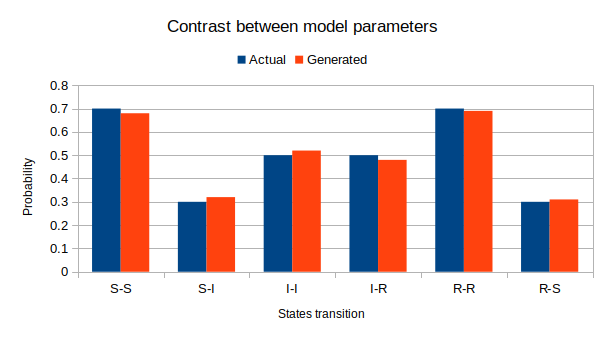
\includegraphics[scale=1]{modelparams.png}
	\caption{Model Parameters}
	\label{fig:mod}
\end{figure}

\subsection{ Goodness of Fit among two models}
If the algorithm learns from the data well then the distance between actual model parameters and learned model parameters should be small and unbiased. For this, we use \textbf{R-Squared} metrics to evaluate how well the generated parameters fit the actual model parameters. R-Squared is always between 0 and 1. 0 means the algorithm learns none of the variability of the actual model parameters. 1 indicates that the model explains all the variability of the model parameters. Generally, the higher the R-squared, the better the model.
 Table[2] below show the model parameters and the R-Squared score which is very close to 1. In conclusion, we can say that the generated model fits the actual parameters very well and they are identical.
%\ref{table:param} 
\begin{table}[h!]
	\centering
	\label{table:param}
	\caption{Model Parameters}
	\begin{tabular}{|l|l|l|}
		\hline
		& \textbf{Actual} & \textbf{Generated} \\ \hline
		\textbf{S-S} & 0.7             & 0.68               \\ \hline
		\textbf{S-I} & 0.3             & 0.32               \\ \hline
		\textbf{I-I} & 0.5             & 0.52               \\ \hline
		\textbf{I-R} & 0.5             & 0.48               \\ \hline
		\textbf{R-R} & 0.7             & 0.69               \\ \hline
		\textbf{R-S} & 0.3             & 0.31               \\ \hline
	\end{tabular}
\end{table}

\begin{equation}
\begin{gathered}
\text{R-Squared} = \frac{\text{Explained variation in model parameters}}{\text{Total variation in actual parameters}} \\
\text{R-Squared for the model} = 0.98875
\end{gathered}
\end{equation}


\subsection{Divergence in steady state distribution of the two model}
Due to the stochastic nature of this modeling stack, we also evaluate the steady-state distribution of both the models to evaluate how similar are generated distribution and actual distribution. We use \textbf{Kullback–Leibler divergence} which is the measure of relative entropy in the probability distribution of the two models. If the two distributions are identical then the Kullback–Leibler divergence between them is very close to 0. Figure \ref{fig:dist} below shows the steady-state distribution of mass for both the models among groups. The distribution is identical and they also have very low divergence value in the equation [\ref{eq:2}]. Perhaps these two models produce similar steady-state distributions and are identical. 
\begin{figure}[h!]
	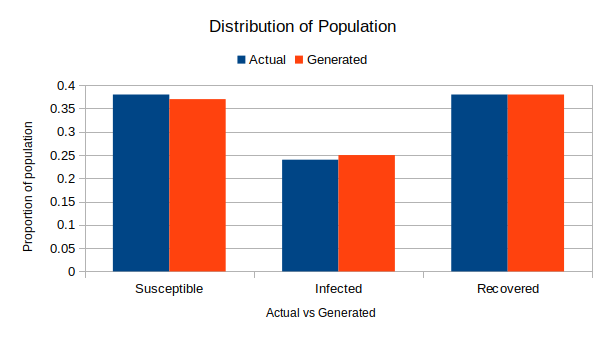
\includegraphics[scale=1]{proportionCompare.png}
	\caption{Steady state distribution}
	\label{fig:dist}
\end{figure}
\begin{equation}\label{eq:2}
\begin{gathered}
D_{KL} (p||q) = E[\log(p(x)) - \log(q(x))] \\
D_{KL} (Actual||Generated) =  0.00034
\end{gathered}
\end{equation}

\subsection{Statistical Test on model outputs}
One of the key advantages of the simulation engine like \textbf{PRAM} is that we can learn the rule from data and use the generated rule directly in the simulator to generate the model output and compare it directly with the actual rule output. The simulation output is the count of the population in each group at every time step. For the evaluation and comparison of two simulation output we use the \textbf{Chi-square test ($\chi^2$)}. The purpose of the Chi-square test is to determine whether the observed count of the population from the auto-generated rule differs from the count of population generated from the actual rule.
\begin{equation}
\chi^2 = \sum_{group}\frac{(Observed_{group} - Actual_{group})^2}{Actual_{group}}
\end{equation}
\subsubsection{Setup} 

\begin{itemize}
	\item In our case of the SIR model we setup the simulation for 20-time steps with an initial population count of 1000 in susceptible \textbf{S} state.
	\item We set up the null Hypothesis $H_0$  and alternate hypothesis $H_A$.
		\subitem $H_0$ : The observed population in each category matches the actual population
		\subitem $H_A$ : The observed population in each category does not match the actual population
	\item We run the simulation for both actual rule and auto-generated rule and then record the count of population in each group at the end of simulation.
	\begin{table}[h!]
		\centering
		\label{table:counts}
		\caption{Model Output}
		\begin{tabular}{|l|l|l|}
			\hline
			& Actual count & Generated count \\ \hline
			S & 384.6        & 369.9           \\ \hline
			I & 230.8        & 247.1           \\ \hline
			R & 384.6        & 383             \\ \hline
		\end{tabular}
	\end{table}
	\item We run the Chi-square test on the population counts and compute the \textit{p-value} with a significance level $\alpha = 0.05$
	\begin{equation}
	\begin{gathered}
	\chi^2 = 1.666\\
	p-value = 0.434
	\end{gathered}
	\end{equation}
	\item Based on the resulting \textit{p-value} we reject or accept the null hypothesis $H_0$
	\subitem Since the \textit{p-value} is greater than significance level $\alpha =0.05$ we fail to reject the $H_0$ 
	\item We can conclude that the population count in every group in both models is identical.
\end{itemize}
With the help of the Chi-squared test, we can conclude that indeed both the model produces identical population distribution among the groups and behave similarly. Thus the rule learned from data is similar to an actual rule created by the modeler


%----------------------------------------------------------------------------------------
% Conclusion
%----------------------------------------------------------------------------------------

\section{Conclusion}
Rule learning will be a very useful tool to automatically generate models from data. This algorithm is useful for non-computer scientists with little knowledge of how the underlying system works and instead has just access to observations to construct a model that represents the system under study. We demonstrated a use case of rule extraction for \textbf{SIR} flu model and we were able to generate the parameters back from data generated by the actual rule. We also evaluated the performance of the rule generator algorithm which confirms that the algorithm can generate accurate models from historical data.
We will expand the capabilities of the algorithm to learn multidimensional rules with even more convoluted relationships between them.



%----------------------------------------------------------------------------------------
% Bibliography
%----------------------------------------------------------------------------------------
\newpage % Includes a new page

\pagenumbering{roman} % Changes page numbering to roman page numbers
%\bibliography{literature}

\bibliography{literature} % Add the filename of your bibliography
\bibliographystyle{apsr} % Defines your bibliography style

% For citing, please see this sheet: http://merkel.texture.rocks/Latex/natbib.php


\end{document}
